\documentclass{article}
\usepackage{fancyhdr} % Required for custom headers
\usepackage{lastpage} % Required to determine the last page for the footer
\usepackage{extramarks} % Required for headers and footers
\usepackage[usenames,dvipsnames]{color} % Required for custom colors
\usepackage{graphicx} % Required to insert images
\usepackage{listings} % Required for insertion of code
\usepackage{courier} % Required for the courier font
\usepackage{lipsum} % Used for inserting dummy 'Lorem ipsum' text into the template
\usepackage{caption}
\usepackage{subcaption}
\usepackage{amsmath}
\usepackage{amsfonts}
\usepackage{amssymb}
\usepackage{epstopdf}
\usepackage{placeins}
\usepackage{color} 
\usepackage{fancyvrb} 
\usepackage{setspace}
\usepackage{array}
\usepackage[numbered]{bookmark}
\usepackage{tikz}
\usepackage{pgfplots}
\usepackage[absolute,overlay]{textpos}
\usetikzlibrary{calc, angles,quotes}
\usetikzlibrary{pgfplots.fillbetween, backgrounds}
\usetikzlibrary{positioning}
\usetikzlibrary{arrows}
\usetikzlibrary{pgfplots.groupplots}
\usetikzlibrary{arrows.meta}
\usetikzlibrary{plotmarks}
\usetikzlibrary{decorations.markings}

\usepgfplotslibrary{groupplots}
\pgfplotsset{compat=newest} 
%\pgfplotsset{plot coordinates/math parser=false}
\DeclareGraphicsExtensions{.pdf,.png,.jpg}
\graphicspath{{figs/}}

\definecolor{matlabcomment}{RGB}{34,139,34}

\pgfmathdeclarefunction{gauss}{1}{%
	\pgfmathparse{1/(sqrt(2*pi))*exp(-((#1)^2)/2)}%
}

\pgfmathdeclarefunction{laplacian}{2}{%
	\pgfmathparse{1/(#2*2)*exp(-(abs(x-#1))/(#2))}%
}

\pgfmathdeclarefunction{pretty_func}{1}{%
	\pgfmathparse{cos(deg(#1/2)) - sin(deg(#1)) + cos(deg(#1/2)-45) - sin(deg(#1/4)-154)}%
}

\pgfplotsset{
	dirac/.style={
		mark=triangle*,
		mark options={scale=2},
		ycomb,
		scatter,
		visualization depends on={y/abs(y)-1 \as \sign},
		scatter/@pre marker code/.code={\scope[rotate=90*\sign,yshift=-2pt]}
	}
}

\def\thickness{very thick}

\tikzset{
amark/.style 2 args={
	decoration={             
		markings, 
		mark=at position {0.5} with { 
			\arrow{stealth},
			\node[#2] {#1};
		}
	}, \thickness,
	postaction={decorate}
},
earlymark/.style 2 args={
	decoration={             
		markings, 
		mark=at position {0.25} with { 
			\arrow{stealth},
			\node[#2] {#1};
		}
	}, \thickness,
	postaction={decorate}
},
latemark/.style 2 args={
	decoration={             
		markings, 
		mark=at position {0.8} with { 
			\arrow{stealth},
			\node[#2] {#1};
		}
	}, \thickness,
	postaction={decorate}
},
zpath/.style={
	decoration={             
		markings, 
		mark=at position {0.5} with { 
			\arrow{stealth},
			\node[#1] {$z^{-1}$};
		}
	}, \thickness,
	postaction={decorate}
},
terminal/.style 2 args={draw,circle,inner sep=2pt,label={#1:#2}},
}


\tikzset{
	invisible/.style={opacity=0},
	visible on/.style={alt={#1{}{invisible}}},
	alt/.code args={<#1>#2#3}{%
		\alt<#1>{\pgfkeysalso{#2}}{\pgfkeysalso{#3}} % \pgfkeysalso doesn't change the path
	},
}

\newcommand\PlotSampledSpectrum[4]{%
	\def\fs{#2}%
	\def\fmax{#3}%
	\def\ros{#4}%
	\input{#1}%
}

\pgfmathdeclarefunction{invgauss}{2}{%
	\pgfmathparse{sqrt(-2*ln(#1))*cos(deg(2*pi*#2))}%
}

\tikzset{
	declare function={
		sinc(\x) = (and(\x!=0, 1) * (sin(deg(pi*\x))/(pi*\x)) +
		(and(\x==0, 1) * 1);
	}
}

\DeclareMathOperator{\E}{\mathbb{E}} % expectation

\newcommand\SimpleSys[4]{%
	\def\xin{#2}%
	\def\Hz{#3}%
	\def\yout{#4}
	\input{#1}%
}

% Margins
\topmargin=-0.45in
\evensidemargin=0in
\oddsidemargin=0in
\textwidth=6.5in
\textheight=9.0in
\headsep=0.25in

\linespread{1.2} % Line spacing

% Set up the header and footer
\pagestyle{fancy}
\lhead{\hmwkAuthorName} % Top left header
\chead{\hmwkTitle} % Top center head
\rhead{\hmwkClass} % Top right header
\lfoot{} % Bottom left footer
\cfoot{} % Bottom center footer
\rfoot{Page\ \thepage\ of\ \protect\pageref{LastPage}} % Bottom right footer
\renewcommand\headrulewidth{0.4pt} % Size of the header rule
\renewcommand\footrulewidth{0.4pt} % Size of the footer rule

%\setlength\parindent{0pt} % Removes all indentation from paragraphs
\definecolor{MyDarkGreen}{rgb}{0.0,0.4,0.0} % This is the color used for comments
\lstloadlanguages{Perl} % Load Perl syntax for listings, for a list of other languages supported see: ftp://ftp.tex.ac.uk/tex-archive/macros/latex/contrib/listings/listings.pdf
\lstset{language=Perl, % Use Perl in this example
        frame=single, % Single frame around code
        basicstyle=\small\ttfamily, % Use small true type font
        keywordstyle=[1]\color{Blue}\bf, % Perl functions bold and blue
        keywordstyle=[2]\color{Purple}, % Perl function arguments purple
        keywordstyle=[3]\color{Blue}\underbar, % Custom functions underlined and blue
        identifierstyle=, % Nothing special about identifiers                                         
        commentstyle=\usefont{T1}{pcr}{m}{sl}\color{MyDarkGreen}\small, % Comments small dark green courier font
        stringstyle=\color{Purple}, % Strings are purple
        showstringspaces=false, % Don't put marks in string spaces
        tabsize=5, % 5 spaces per tab
        %
        % Put standard Perl functions not included in the default language here
        morekeywords={rand},
        %
        % Put Perl function parameters here
        morekeywords=[2]{on, off, interp},
        %
        % Put user defined functions here
        morekeywords=[3]{test},
       	%
        morecomment=[l][\color{Blue}]{...}, % Line continuation (...) like blue comment
        numbers=left, % Line numbers on left
        firstnumber=1, % Line numbers start with line 1
        numberstyle=\tiny\color{Blue}, % Line numbers are blue and small
        stepnumber=5 % Line numbers go in steps of 5
}

% Creates a new command to include a perl script, the first parameter is the filename of the script (without .pl), the second parameter is the caption
\newcommand{\perlscript}[2]{
\begin{itemize}
\item[]\lstinputlisting[caption=#2,label=#1]{#1.pl}
\end{itemize}
}

% Header and footer for when a page split occurs within a problem environment
\newcommand{\enterProblemHeader}[1]{
\nobreak\extramarks{#1}{#1 continued on next page\ldots}\nobreak
\nobreak\extramarks{#1 (continued)}{#1 continued on next page\ldots}\nobreak
}

% Header and footer for when a page split occurs between problem environments
\newcommand{\exitProblemHeader}[1]{
\nobreak\extramarks{#1 (continued)}{#1 continued on next page\ldots}\nobreak
\nobreak\extramarks{#1}{}\nobreak
}

\setcounter{secnumdepth}{0} % Removes default section numbers
\newcounter{homeworkProblemCounter} % Creates a counter to keep track of the number of problems

\newcommand{\homeworkProblemName}{}
\newenvironment{homeworkProblem}[1][Problem \arabic{homeworkProblemCounter}]{ % Makes a new environment called homeworkProblem which takes 1 argument (custom name) but the default is "Problem #"
\stepcounter{homeworkProblemCounter} % Increase counter for number of problems
\renewcommand{\homeworkProblemName}{#1} % Assign \homeworkProblemName the name of the problem
\section{\homeworkProblemName} % Make a section in the document with the custom problem count
\enterProblemHeader{\homeworkProblemName} % Header and footer within the environment
}{
\exitProblemHeader{\homeworkProblemName} % Header and footer after the environment
}

\newcommand{\problemAnswer}[1]{ % Defines the problem answer command with the content as the only argument
\noindent\framebox[\columnwidth][c]{\begin{minipage}{0.98\columnwidth}#1\end{minipage}} % Makes the box around the problem answer and puts the content inside
}

\newcommand{\homeworkSectionName}{}
\newenvironment{homeworkSection}[1]{ % New environment for sections within homework problems, takes 1 argument - the name of the section
\renewcommand{\homeworkSectionName}{#1} % Assign \homeworkSectionName to the name of the section from the environment argument
\subsection{\homeworkSectionName} % Make a subsection with the custom name of the subsection
\enterProblemHeader{\homeworkProblemName\ [\homeworkSectionName]} % Header and footer within the environment
}{
\enterProblemHeader{\homeworkProblemName} % Header and footer after the environment
}

%----------------------------------------------------------------------------------------
%	NAME AND CLASS SECTION
%----------------------------------------------------------------------------------------
%%%%%%%%%%%%%%%%%%%%%%%%%%%%%%%%%%%%%%%%%%%%%%%%%%%%%%%%%%%%%%%%%%%%%%%%%%%%%%%%%%%%%%%%%
\newcommand{\hmwkTitle}{Homework \#02} % Assignment title
\newcommand{\hmwkDueDate}{\today} % Due date
\newcommand{\hmwkClass}{EE 264 (Summer 2018)} % Course/class
\newcommand{\hmwkAuthorName}{Solutions} % Your name
%%%%%%%%%%%%%%%%%%%%%%%%%%%%%%%%%%%%%%%%%%%%%%%%%%%%%%%%%%%%%%%%%%%%%%%%%%%%%%%%%%%%%%%%%
%----------------------------------------------------------------------------------------
%	TITLE PAGE
%----------------------------------------------------------------------------------------
\title{
\vspace{2in}
\textmd{\textbf{\hmwkClass:\ \hmwkTitle}}\\
\normalsize\vspace{0.1in}\small{Due\ on\ \hmwkDueDate}\\
\vspace{0.1in}\large{\textit{\hmwkClassInstructor\ \hmwkClassTime}}
\vspace{3in}
}

\author{\textbf{\hmwkAuthorName}}
\date{} % Insert date here if you want it to appear below your name

%----------------------------------------------------------------------------------------

\begin{document}
	
\section{Problem 1}
\subsection{(a)}

\FloatBarrier
\begin{figure}[h!]
	\centering
	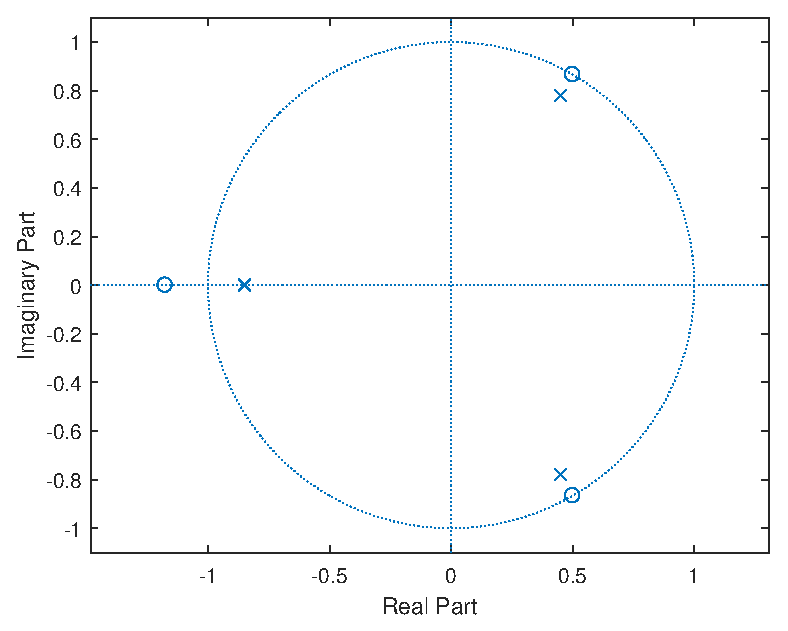
\includegraphics[scale=0.7]{figs/hw4q1a_pole_zero.eps}
	\caption{Zero-pole diagram}
\end{figure}
\FloatBarrier

\subsection{(b)}

\FloatBarrier
\begin{figure}[h!]
	\centering
	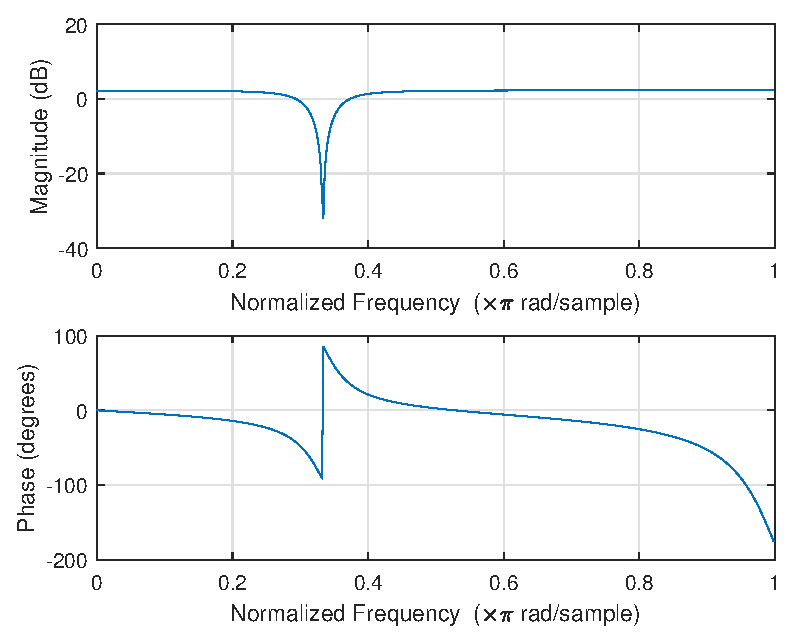
\includegraphics[scale=0.7]{figs/hw4q1b_mag_phase.eps}
	\caption{Magnitude and phase plots}
\end{figure}
\FloatBarrier

\subsection{(c)}

\FloatBarrier
\begin{figure}[h!]
	\centering
	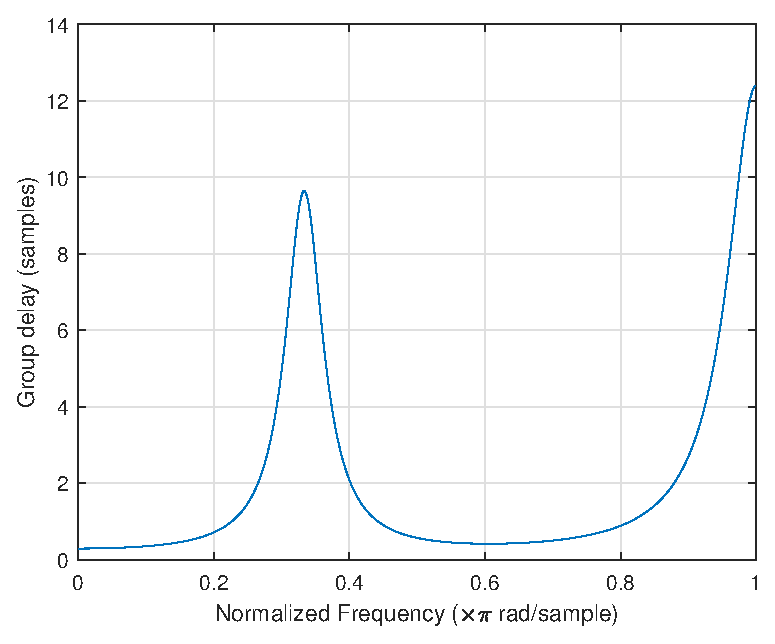
\includegraphics[scale=0.7]{figs/hw4q1b_grpdelay.eps}
	\caption{Group delay}
\end{figure}
\FloatBarrier

\subsection{(d)}

\begin{enumerate}
	\item True. All poles are inside the unit circle.
	\item False. Since the system is stable its impulse response must be absolute summable. Therefore, it cannot converge to a non-zero value when $n\to\infty$.
	\item False. The system also has a zero at that frequency, and that zero is actually on the unit circle, so it has a bigger influence on the frequency response. As a result, the magnitude response has a dip at $\omega = \pi/3$.
	\item False. The system has zeros outside the unit circle.
	\item False. Since the system has a zero outside the unit circle, its inverse is unstable.

\end{enumerate}

\definecolor{mblue}{rgb}{0,0,1} 
\definecolor{mgreen}{rgb}{0.13333,0.5451,0.13333} 
\definecolor{mred}{rgb}{0.62745,0.12549,0.94118} 
\definecolor{mgrey}{rgb}{0.5,0.5,0.5} 
\definecolor{mdarkgrey}{rgb}{0.25,0.25,0.25} 
  
\DefineShortVerb[fontfamily=courier,fontseries=m]{\$} 
\DefineShortVerb[fontfamily=courier,fontseries=b]{\#} 
  
\noindent                 
 \hspace*{2.4em}{\scriptsize 1}$  $\color{mgrey}#%% Problem 1 Code - a, b, c#\color{black}$$\\
 \hspace*{2.4em}{\scriptsize 4}$  b = conv(conv([1 -exp(1j*pi/3)], [1 -exp(-1j*pi/3)]), [1 1/0.85]);$\\
 \hspace*{2.4em}{\scriptsize 5}$  a = conv(conv([1 -0.9*exp(1j*pi/3)], [1 -0.9*exp(-1j*pi/3)]), [1 0.85]);$\\
 \hspace*{2.4em}{\scriptsize 6}$  $\\
 \hspace*{2.4em}{\scriptsize 7}$  $\color{mgrey}#%% a)#\color{black}$$\\
 \hspace*{2.4em}{\scriptsize 8}$  zplane(b, $\color{mdarkgrey}$a) $\color{black}$$\color{mgrey}$% b and a must be row vectors$\color{black}$$\\
 \hspace*{2.4em}{\scriptsize 9}$  saveas(gca, $\color{mdarkgrey}$'../figs/hw4q1a_pole_zero'$\color{black}$, $\color{mdarkgrey}$'epsc'$\color{black}$)$\\
 \hspace*{2em}{\scriptsize 10}$  $\\
 \hspace*{2em}{\scriptsize 11}$  $\color{mgrey}#%% b)#\color{black}$$\\
 \hspace*{2em}{\scriptsize 12}$  figure, $\color{mdarkgrey}$freqz(b, a)$\color{black}$$\\
 \hspace*{2em}{\scriptsize 13}$  saveas(gca, $\color{mdarkgrey}$'../figs/hw4q1b_mag_phase'$\color{black}$, $\color{mdarkgrey}$'epsc'$\color{black}$)$\\
 \hspace*{2em}{\scriptsize 14}$  $\\
 \hspace*{2em}{\scriptsize 15}$  $\color{mgrey}#%% c)#\color{black}$$\\
 \hspace*{2em}{\scriptsize 16}$  figure, $\color{mdarkgrey}$grpdelay(b, a)$\color{black}$$\\
 \hspace*{2em}{\scriptsize 17}$  saveas(gca, $\color{mdarkgrey}$'../figs/hw4q1b_grpdelay'$\color{black}$, $\color{mdarkgrey}$'epsc'$\color{black}$)$\\ 
  
\UndefineShortVerb{\$} 
\UndefineShortVerb{\#}





\newpage

\section{Problem 2}
\subsection{(a)}

\begin{figure}[!h]
	\resizebox{0.9\textwidth}{!}{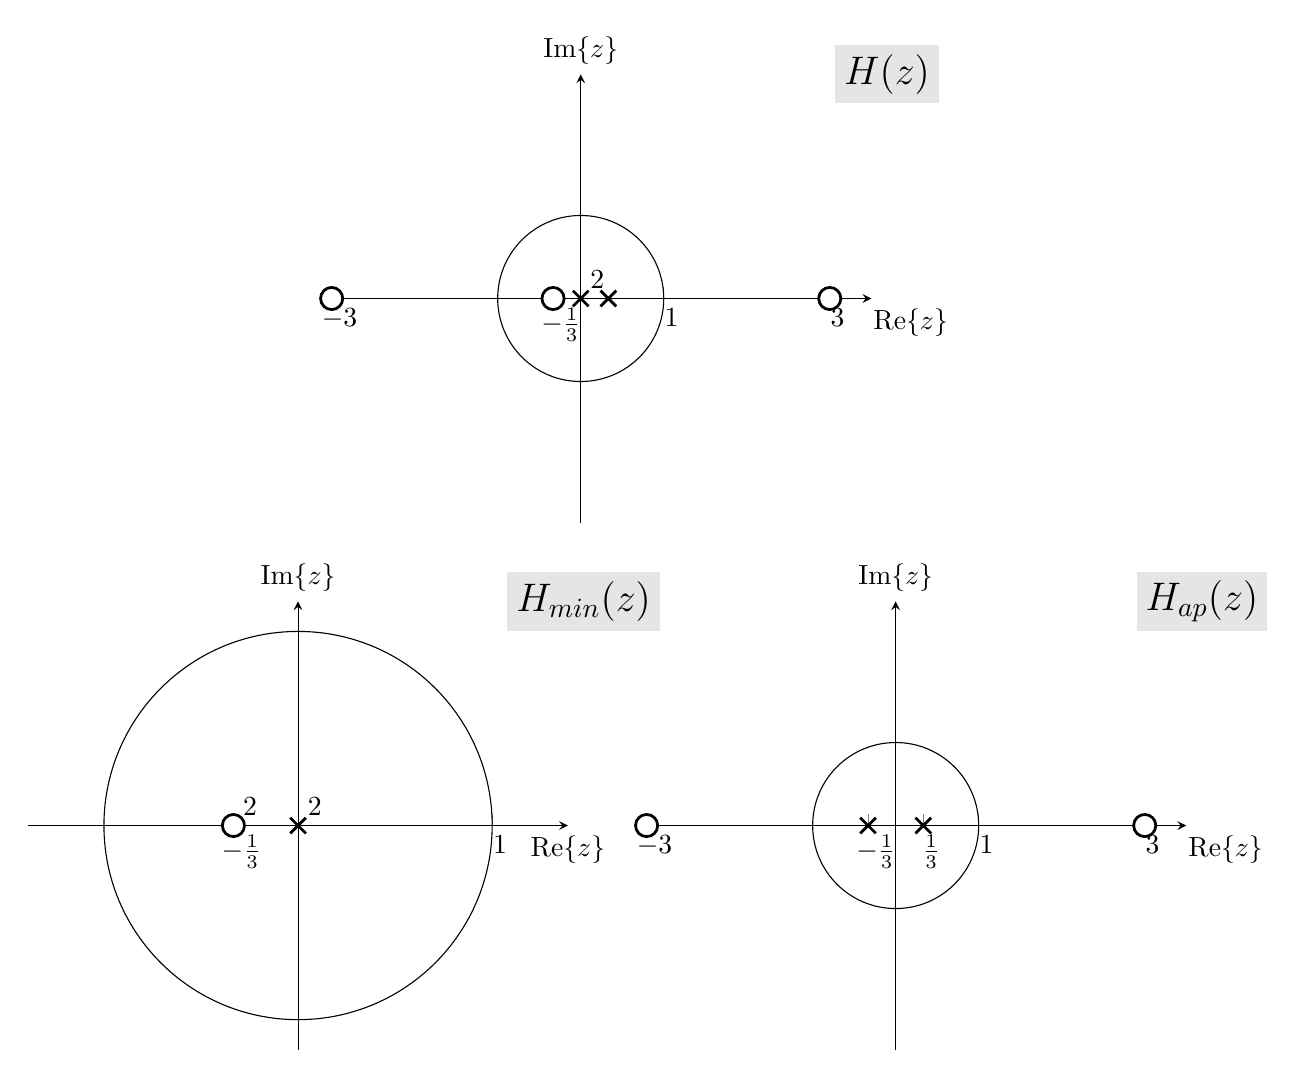
\begin{tikzpicture}
\begin{axis}[
name=plot1,
axis equal,
axis lines*=middle,
enlargelimits = false, clip=true,
xmin=-3,
xmax=3.5,
ymin=-1.10,
ymax=1.10,
axis line style={->,>=stealth},
xlabel={$\mathrm{Re}\{z\}$},
ylabel={$\mathrm{Im}\{z\}$},
every axis x label/.style={
at={(ticklabel* cs:1)},
anchor=north,
xshift=0.5cm,
},
every axis y label/.style={
at={(ticklabel* cs:1)},
anchor=south,
},
xtick={-3, -0.333, 3, 1}, xticklabels={$-3$, $-\frac{1}{3}$, $3$, 1}, ytick=\empty,
xticklabel style={xshift=0.1cm},
every outer y axis line/.append style={white!15!black},
every y tick label/.append style={font=\color{white!15!black}},
legend style={draw=white!15!black,fill=white,legend cell align=left}]
\draw (axis cs:0,0) circle [black!50, dashed, line width=2pt, radius=1];
\addplot [line width=1pt,mark=x, only marks, mark size = 4pt]
table[row sep=crcr]{
 0 0 \\
 0.333 0 \\
};

\addplot [line width=1pt,mark=*, only marks, mark size = 4pt, mark options={fill=white}]
table[row sep=crcr]{
	-3 0 \\
	3 0 \\
	-0.3333 0\\
};
\node[above, anchor=south west] at (axis cs: 0, 0) {$2$};
\end{axis}

\begin{axis}[
name=plot2,
at= (plot1.south west), anchor=north east, xshift=3cm, yshift=-1cm,
%at=(plot1.below south east), anchor=above north east,
axis equal,
axis lines*=middle,
enlargelimits = false, clip=true,
xmin=-1.39,
xmax=1.39,
ymin=-1.10,
ymax=1.10,
axis line style={->,>=stealth},
xlabel={$\mathrm{Re}\{z\}$},
ylabel={$\mathrm{Im}\{z\}$},
every axis x label/.style={
	at={(ticklabel* cs:1)},
	anchor=north,
},
every axis y label/.style={
	at={(ticklabel* cs:1)},
	anchor=south,
},
xtick={-0.333, 1}, xticklabels={$-\frac{1}{3}$, $1$}, ytick=\empty,
xticklabel style={xshift=0.1cm},
every outer y axis line/.append style={white!15!black},
every y tick label/.append style={font=\color{white!15!black}},
legend style={draw=white!15!black,fill=white,legend cell align=left}]
\draw (axis cs:0,0) circle [black!50, dashed, line width=2pt, radius=1];
\addplot [line width=1pt,mark=x, only marks, mark size = 4pt]
table[row sep=crcr]{
	 0 0 \\
};

\addplot [line width=1pt,mark=*, only marks, mark size = 4pt, mark options={fill=white}]
table[row sep=crcr]{
	-0.333 0 \\
};
\node[above, anchor=south west] at (axis cs: -0.333, 0) {$2$};
\node[above, anchor=south west] at (axis cs: 0, 0) {$2$};
\end{axis}

\begin{axis}[
name=plot3,
at= (plot2.east), anchor=west, xshift=1cm,
%at=(plot2.below south east), anchor=above north east,
axis equal,
axis lines*=middle,
enlargelimits = false, clip=true,
xmin=-3,
xmax=3.5,
ymin=-1.10,
ymax=1.10,
axis line style={->,>=stealth},
xlabel={$\mathrm{Re}\{z\}$},
ylabel={$\mathrm{Im}\{z\}$},
every axis x label/.style={
	at={(ticklabel* cs:1)},
	anchor=north,
	xshift=0.5cm,
},
every axis y label/.style={
	at={(ticklabel* cs:1)},
	anchor=south,
},
xtick={-3, -0.333, 0.333, 3, 1}, xticklabels={$-3$, $-\frac{1}{3}$, $\frac{1}{3}$, $3$, 1}, ytick=\empty,
xticklabel style={xshift=0.1cm},
every outer y axis line/.append style={white!15!black},
every y tick label/.append style={font=\color{white!15!black}},
legend style={draw=white!15!black,fill=white,legend cell align=left}]
\draw (axis cs:0,0) circle [black!50, dashed, line width=2pt, radius=1];
\addplot [line width=1pt,mark=x, only marks, mark size = 4pt]
table[row sep=crcr]{
	-0.333 0 \\
	0.333 0 \\
};

\addplot [line width=1pt,mark=*, only marks, mark size = 4pt, mark options={fill=white}]
table[row sep=crcr]{
	-3 0 \\
	3 0 \\
};
\end{axis}
\node[black, fill=black!10, minimum width=1cm, align=center] at ($(plot1.north east)+(0.2cm,0)$) {\Large $H(z)$};
\node[black, fill=black!10, minimum width=1cm, align=center] at ($(plot2.north east)+(0.2cm,0)$) {\Large $H_{min}(z)$};
\node[black, fill=black!10, minimum width=1cm, align=center] at ($(plot3.north east)+(0.2cm,0)$) {\Large $H_{ap}(z)$};

\end{tikzpicture}}
\end{figure}

We must follow this algorithm:
\begin{enumerate}
	\item In the minimum phase system, reflect all zeros outside the unit circle to their reciprocal conjugate.
	\item In the all-pass system, add poles at the reciprocal conjugate of the zeros outside the unit circle
	\item (optional) Adjust gain of the minimum phase system to match the gain of the original system, so that the all-pass system has unit gain.
\end{enumerate}

Therefore,
\begin{equation}
H_{min}(z) = -9(1 + 1/3z^{-1})^2
\end{equation}

\begin{equation}
H_{ap}(z) = -\frac{1}{9}\frac{(1 + 3z^{-1})(1 - 3z^{-1})}{(1 + 1/3z^{-1})(1 - 1/3z^{-1})}
\end{equation}
	
This choice is unique up to a scale factor.
	
\subsection{(b)}
Yes, it has all poles at the origin.

\subsection{(c)}

Since the filter has real coefficients, if $c$ is a zero, $c^*$ must also be a zero.

Due to the symmetry conditions, causal generalized linear phase FIR systems must obey one of following relations:
\begin{align*}
H(z) = z^MH(z^{-1}) \tag{if even symmetric} \\
H(z) = -z^MH(z^{-1}) \tag{if odd symmetric} \\
\end{align*}

Therefore, if $c$ is a zero, $1/c$ must also be a zero:

\begin{align*}
H(c) = 0 = \pm c^MH(c^{-1})
\end{align*}

Again, from the real coefficients condition, if $1/c$ is a zero, $1/c^*$ must also be a zero.

Therefore, if $c$ is a zero, $c^*, 1/c, 1/c^*$ must also be zeros.

\noindent\textbf{Note:} this result can also be extended to other systems with real coefficients and even/odd symmetry. First, if a system (FIR or not) has real coefficients, its poles and zeros will appear as complex conjugate pairs. This follows from algebra, since the roots of a polynomial with real coefficients are either real or appear in complex conjugate pairs. Second, if a system (FIR or not) has even or odd symmetry, the poles and zeros will appear as conjugate reciprocal pairs. This follows from the properties of the $z$-transform:
\begin{align}
h[n] = \pm h[-n] \tag{even or odd symmetry} \\
H(z) = \pm H(z^{-1}) \tag{time reversal property of the $z$-transform}
\end{align}
Therefore, if $c$ is a zero of $H(z)$, $1/c$ must also be a zero of $H(z)$, since $H(z = 1/c) = H(z = c) = 0$. Analogously, if $p$ is a pole of $H(z)$, $1/p$ must also be a pole of $H(z)$, since $H(z = 1/p) = H(z = p) = \infty$.

\subsection{(d)}

Using the result from part (c), we can do the following decomposition:

\begin{figure}[!h]
	\resizebox{0.9\textwidth}{!}{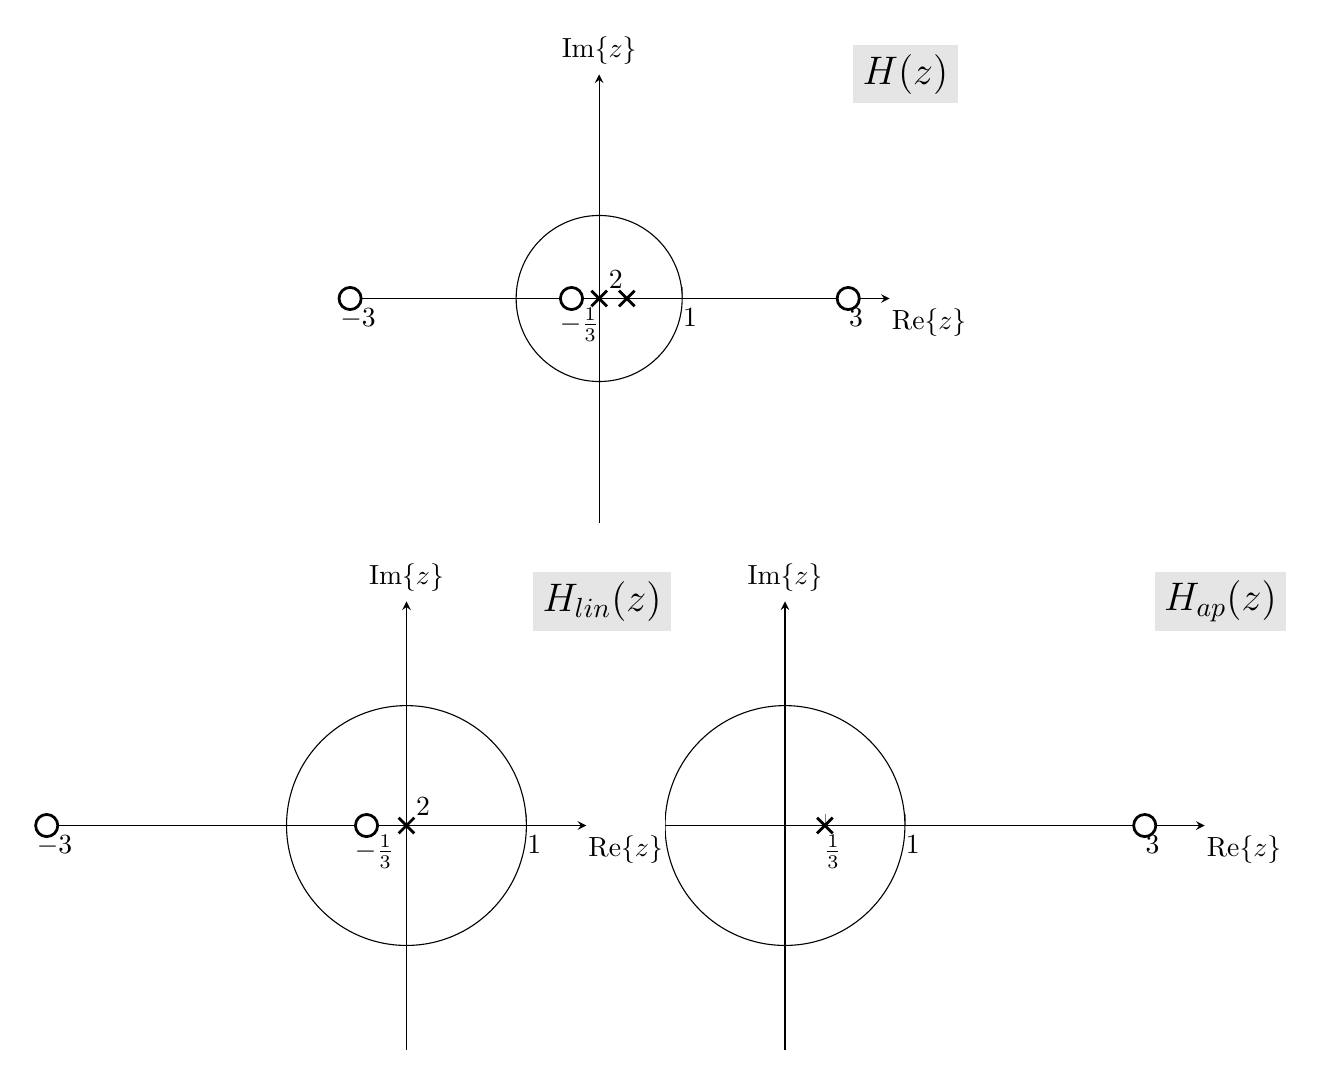
\begin{tikzpicture}
\begin{axis}[
name=plot1,
axis equal,
axis lines*=middle,
enlargelimits = false, clip=true,
xmin=-3,
xmax=3.5,
ymin=-1.10,
ymax=1.10,
axis line style={->,>=stealth},
xlabel={$\mathrm{Re}\{z\}$},
ylabel={$\mathrm{Im}\{z\}$},
every axis x label/.style={
at={(ticklabel* cs:1)},
anchor=north,
xshift=0.5cm,
},
every axis y label/.style={
at={(ticklabel* cs:1)},
anchor=south,
},
xtick={-3, -0.333, 3, 1}, xticklabels={$-3$, $-\frac{1}{3}$, $3$, 1}, ytick=\empty,
xticklabel style={xshift=0.1cm},
every outer y axis line/.append style={white!15!black},
every y tick label/.append style={font=\color{white!15!black}},
legend style={draw=white!15!black,fill=white,legend cell align=left}]
\draw (axis cs:0,0) circle [black!50, dashed, line width=2pt, radius=1];
\addplot [line width=1pt,mark=x, only marks, mark size = 4pt]
table[row sep=crcr]{
 0 0 \\
 0.333 0 \\
};

\addplot [line width=1pt,mark=*, only marks, mark size = 4pt, mark options={fill=white}]
table[row sep=crcr]{
	-3 0 \\
	3 0 \\
	-0.3333 0\\
};
\node[above, anchor=south west] at (axis cs: 0, 0) {$2$};
\end{axis}

\begin{axis}[
name=plot2,
at= (plot1.south west), anchor=north east, xshift=3cm, yshift=-1cm,
%at=(plot1.below south east), anchor=above north east,
axis equal,
axis lines*=middle,
enlargelimits = false, clip=true,
xmin=-3,
xmax=1.5,
ymin=-1.10,
ymax=1.10,
axis line style={->,>=stealth},
xlabel={$\mathrm{Re}\{z\}$},
ylabel={$\mathrm{Im}\{z\}$},
every axis x label/.style={
	at={(ticklabel* cs:1)},
	anchor=north,
	xshift=0.5cm,
},
every axis y label/.style={
	at={(ticklabel* cs:1)},
	anchor=south,
},
xtick={-3, -0.333, 1}, xticklabels={$-3$, $-\frac{1}{3}$, $1$}, ytick=\empty,
xticklabel style={xshift=0.1cm},
every outer y axis line/.append style={white!15!black},
every y tick label/.append style={font=\color{white!15!black}},
legend style={draw=white!15!black,fill=white,legend cell align=left}]
\draw (axis cs:0,0) circle [black!50, dashed, line width=2pt, radius=1];
\addplot [line width=1pt,mark=x, only marks, mark size = 4pt]
table[row sep=crcr]{
	 0 0 \\
};

\addplot [line width=1pt,mark=*, only marks, mark size = 4pt, mark options={fill=white}]
table[row sep=crcr]{
	-0.333 0 \\
	-3 0 \\
};
\node[above, anchor=south west] at (axis cs: 0, 0) {$2$};
\end{axis}

\begin{axis}[
name=plot3,
at= (plot2.east), anchor=west, xshift=1cm,
%at=(plot2.below south east), anchor=above north east,
axis equal,
axis lines*=middle,
enlargelimits = false, clip=true,
xmin=-1,
xmax=3.5,
ymin=-1.10,
ymax=1.10,
axis line style={->,>=stealth},
xlabel={$\mathrm{Re}\{z\}$},
ylabel={$\mathrm{Im}\{z\}$},
every axis x label/.style={
	at={(ticklabel* cs:1)},
	anchor=north,
	xshift=0.5cm,
},
every axis y label/.style={
	at={(ticklabel* cs:1)},
	anchor=south,
},
xtick={0.333, 3, 1}, xticklabels={$\frac{1}{3}$, $3$, 1}, ytick=\empty,
xticklabel style={xshift=0.1cm},
every outer y axis line/.append style={white!15!black},
every y tick label/.append style={font=\color{white!15!black}},
legend style={draw=white!15!black,fill=white,legend cell align=left}]
\draw (axis cs:0,0) circle [black!50, dashed, line width=2pt, radius=1];
\addplot [line width=1pt,mark=x, only marks, mark size = 4pt]
table[row sep=crcr]{
	0.333 0 \\
};

\addplot [line width=1pt,mark=*, only marks, mark size = 4pt, mark options={fill=white}]
table[row sep=crcr]{
	3 0 \\
};
\end{axis}
\node[black, fill=black!10, minimum width=1cm, align=center] at ($(plot1.north east)+(0.2cm,0)$) {\Large $H(z)$};
\node[black, fill=black!10, minimum width=1cm, align=center] at ($(plot2.north east)+(0.2cm,0)$) {\Large $H_{lin}(z)$};
\node[black, fill=black!10, minimum width=1cm, align=center] at ($(plot3.north east)+(0.2cm,0)$) {\Large $H_{ap}(z)$};

\end{tikzpicture}}
\end{figure}

Therefore,
\begin{equation}
H_{lin}(z) = (1 + 3z^{-1})(1 +1/3z^{-1})
\end{equation}

\begin{equation}
H_{ap}(z) = -\frac{1 - 3z^{-1}}{1 - 1/3z^{-1}}
\end{equation}

\FloatBarrier
\begin{figure}[h!]
	
\end{figure}
\FloatBarrier
\newpage

\section{Problem 3}
\begin{description}
	\item[(a)] A, B, and E. All their poles are at the origin.
	\item[(b)] All. All of them have all poles inside the unit circle.
	\item[(c)] F. It's the only system that appears to have zeros located at the conjugate symmetric of its poles i.e., if $e_k$ is a pole, then $1/e_k^*$ must be a zero.
	\item[(d)] E. All its zeros are inside the unit circle. [D is also acceptable as no zeroes are outside the unit circle.]
	\item[(e)] A and B. Their zeros appear in conjugate pairs and conjugate reciprocal pairs.
	\item[(f)] A and D. They have zeros at $z = -1$, which corresponds to $\omega = \pm\pi$.
	\item[(g)] A and D. Their maximum frequency response appears at low frequencies. In A for the absence of zeros close to $\omega =0$, and in D the poles near  $\omega =0$ increase the magnitude response.
	\item[(h)] E. It's the FIR system with the fewest number of zeros (poles).
	\item[(i)] E. It's the only minimum phase system.
	\item[(j)] 
	\begin{align}\nonumber
	H(z) &= \frac{(1 + 1.1z^{-1})(1 - 1.1z^{-1})}{(1 + 0.8z^{-1})(1 -0.8z^{-1})} \\
	&=\underbrace{\frac{(1 + 1/1.1z^{-1})(1 - 1/1.1z^{-1})}{(1 + 0.8z^{-1})(1 -0.8z^{-1})}}_{H_{min}(z)}\cdot\underbrace{\frac{(1 + 1.1z^{-1})(1 - 1.1z^{-1})}{(1 + 1/1.1z^{-1})(1 -1.1z^{-1})}}_{H_{ap}(z)}
	\end{align}
	
\end{description}	

\mbox{}\\ 
	
\section{Problem 4: Kramers-Kronig relations in discrete time}
\subsection{(a)}

Using the time reversal property of real signals
\begin{equation}
x[-n] \Longleftrightarrow X^*(e^{j\omega}) \tag{time reversal of real signals}
\end{equation}

We can write:
\begin{align}
	X_e(e^{j\omega}) &= \frac{1}{2}\Big(X(e^{j\omega}) + X^*(e^{j\omega})\Big) = \mathrm{Re}\{X(e^{j\omega})\} \\
	X_o(e^{j\omega}) &= \frac{1}{2}\Big(X(e^{j\omega}) - X^*(e^{j\omega})\Big) = j\mathrm{Im}\{X(e^{j\omega})\} 
\end{align}

These results indicate that for real-valued signals, even symmetry in time domain corresponds to purely real frequency component, whereas odd symmetry in time domain corresponds to purely imaginary frequency component. This relationship stems from the fact that $e^{j\omega} = \cos\omega + j\sin\omega$, cosine is a even function and sine is an odd function.

This result is also valid for continuous-time signals.
\subsection{(b)}

Since $x[n] = x_e[n] + x_o[n]$, and since $x[n]$ is causal i.e., $x[n] = 0, n < 0$, we must have that

\begin{equation}
x_o[n] = -x_e[n], n < 0 \implies x[n] = 0, n < 0
\end{equation}

By definition $x_o[n]$ is odd symmetric: $x_o[n] = -x_o[-n]$. Therefore,
\begin{align} \nonumber
x_o[n] &= \begin{cases}
x_e[n], &n > 0 \\
0, & n = 0 \\
-x_e[n], &n < 0
\end{cases} \\
&= \mathrm{sign}[n]x_e[n],
\end{align}
where the sign function is simply
\begin{equation}
\mathrm{sign}[n] = \begin{cases}
1, &n > 0 \\
0, & n = 0 \\
-1, & n < 0
\end{cases}
\end{equation}

Multiplication in time domain corresponds to convolution in frequency domain:
\begin{align}
X_o(e^{j\omega}) = \frac{1}{2\pi}\Big(\mathcal{F}\{\mathrm{sign}[n]\}\ast X_e(e^{j\omega})\Big),
\end{align}
Following the hint: $\mathcal{F}\{\mathrm{sign}[n]\} = -j\frac{\sin\omega}{1-\cos\omega}, |\omega| < \pi$. Thus, 
\begin{align}
X_o(e^{j\omega}) = \frac{1}{2\pi}\Big(-j\frac{\sin\omega}{1-\cos\omega}\ast X_e(e^{j\omega})\Big),
\end{align}

\subsection{(c)}

Combining the results from parts (a) and (b):
\begin{align}
X_o(e^{j\omega}) &= \frac{1}{2\pi}\Big(-j\frac{\sin\omega}{1-\cos\omega}\ast X_e(e^{j\omega})\Big) \tag{from part (b)} \\
j\mathrm{Im}\{X(e^{j\omega})\} &= \frac{1}{2\pi}\Big(-j\frac{\sin\omega}{1-\cos\omega}\ast \mathrm{Re}\{X(e^{j\omega})\}\Big) \tag{from part (a)} \\
\mathrm{Im}\{X(e^{j\omega})\} &= -\frac{1}{2\pi}\Big(\frac{\sin\omega}{1-\cos\omega}\ast \mathrm{Re}\{X(e^{j\omega})\}\Big)
\end{align}

\end{document}